%%%%%%%%%%%%
%
% $Autor: Müller, Hinrichs $
% $Datum: 2026-06-20 10:37:32Z $
% $Pfad: UltraschallradarAutomatisierungstechnik/Manuals/Benutzerhandbuch/Chapters/de/Functions.tex $
% $Version: 1 $
% !TeX spellcheck = en_GB/de_DE
% !TeX encoding = utf8
% !TeX root = manual 
% !TeX TXS-program:bibliography = txs:///biber
%
%%%%%%%%%%%%

\chapter{Bedienung und Anzeige}

\section{Das Radar-Bild interpretieren}
\begin{figure}[h]
	\centering
	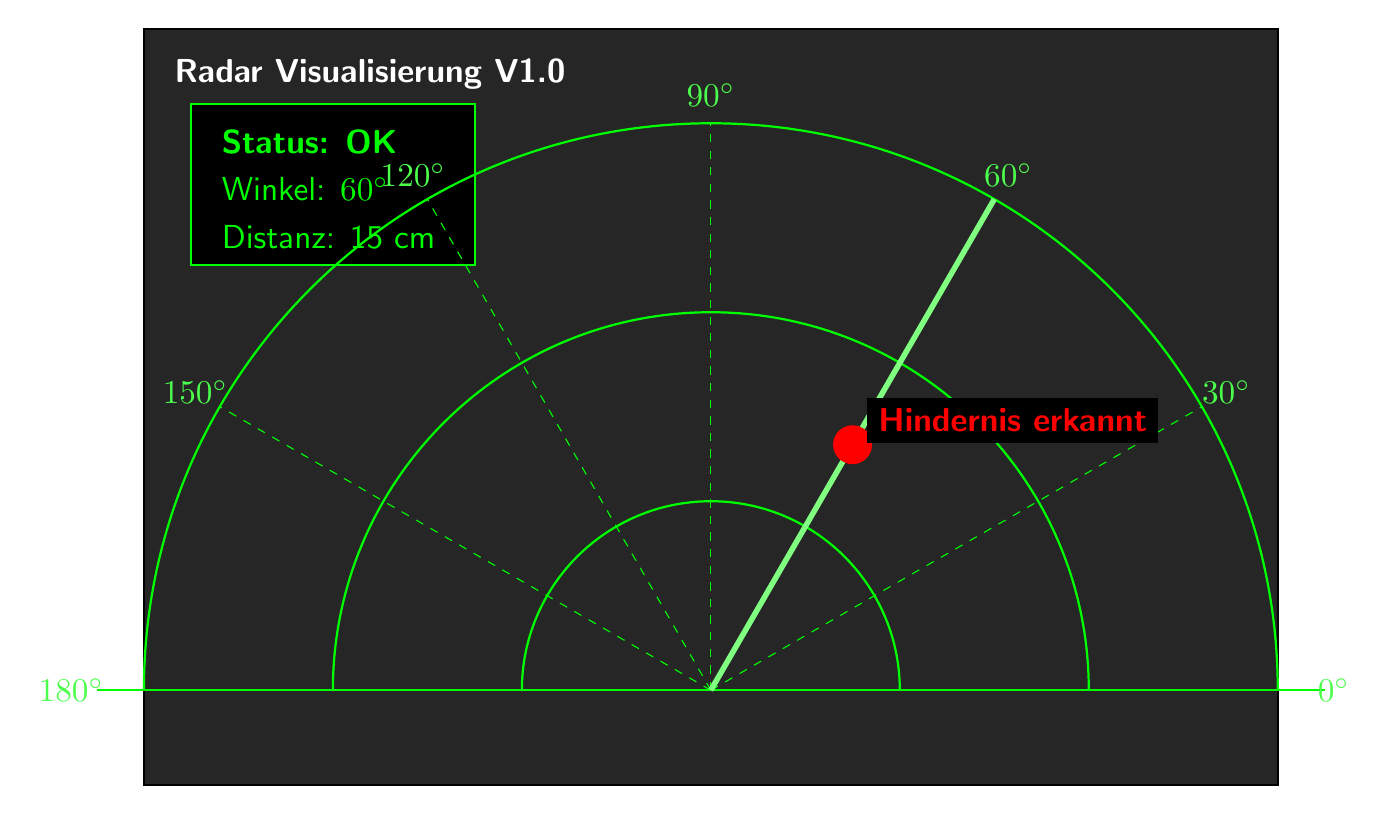
\begin{tikzpicture}[scale=1.2, transform shape, font=\sffamily]
	% Fensterrahmen
	\draw[thick, fill=black!85] (0,0) rectangle (12,8);
	\node[text=white, anchor=north west] at (0.2, 7.8) {\textbf{Radar Visualisierung V1.0}};
	
	% Status Box
	\draw[thick, fill=black, draw=green] (0.5, 5.5) rectangle (3.5, 7.2);
	\node[text=green, anchor=west] at (0.7, 6.8) {\textbf{Status: OK}};
	\node[text=green, anchor=west] at (0.7, 6.3) {Winkel: $60^\circ$};
	\node[text=green, anchor=west] at (0.7, 5.8) {Distanz: 15 cm};
	
	% Radar Gitter (Zentrum bei x=6, y=1)
	\begin{scope}[shift={(6,1)}]
		% Halbkreise (Abstandslinien)
		\foreach \r in {2, 4, 6} {
			\draw[green, thick] (\r,0) arc (0:180:\r);
		}
		% Grundlinie
		\draw[green, thick] (-6.5, 0) -- (6.5, 0);
		
		% Winkellinien
		\foreach \a in {30, 60, 90, 120, 150} {
			\draw[green, dashed] (0,0) -- (\a:6);
			\node[text=green!70, anchor=center] at (\a:6.3) {$\a^\circ$};
		}
		\node[text=green!70, anchor=west] at (6.3, 0) {$0^\circ$};
		\node[text=green!70, anchor=east] at (-6.3, 0) {$180^\circ$};
		
		% Scan-Linie (aktueller Winkel bei 60 Grad)
		\draw[green!50!white, line width=2pt] (0,0) -- (60:6);
		
		% Hindernis (roter Punkt)
		\filldraw[red] (60:3) circle (0.2);
		\node[text=red, right, fill=black] at (60:3.3) {\textbf{Hindernis erkannt}};
	\end{scope}
\end{tikzpicture}
	\caption{Benutzeroberfläche}
\end{figure}

Nach bestandenem Selbsttest wechselt das Radarsystem automatisch in den Normalbetrieb. Die grüne Status-LED am Gehäuse leuchtet nun dauerhaft.

Auf Ihrem Bildschirm sehen Sie eine kreisförmige Anzeige.

\begin{itemize}
	\item \textbf{Visuelle Darstellung:} Das Zentrum der Benutzeroberfläche bildet ein Radar-Gitter in Form von Halbkreisen mit festen Abstands- und Winkelmarkierungen. Ein optischer Scan-Strahl bewegt sich im Halbkreis stufenlos von $0^\circ$ auf $180^\circ$ und wieder zurück.
	\item \textbf{Hindernisse:} Erkannte Hindernisse werden je nach Größe als rote Punkte oder rote Linien auf dem Gitter eingezeichnet.
\end{itemize}

\section{Reichweite}
\begin{figure}[h]
	\centering
	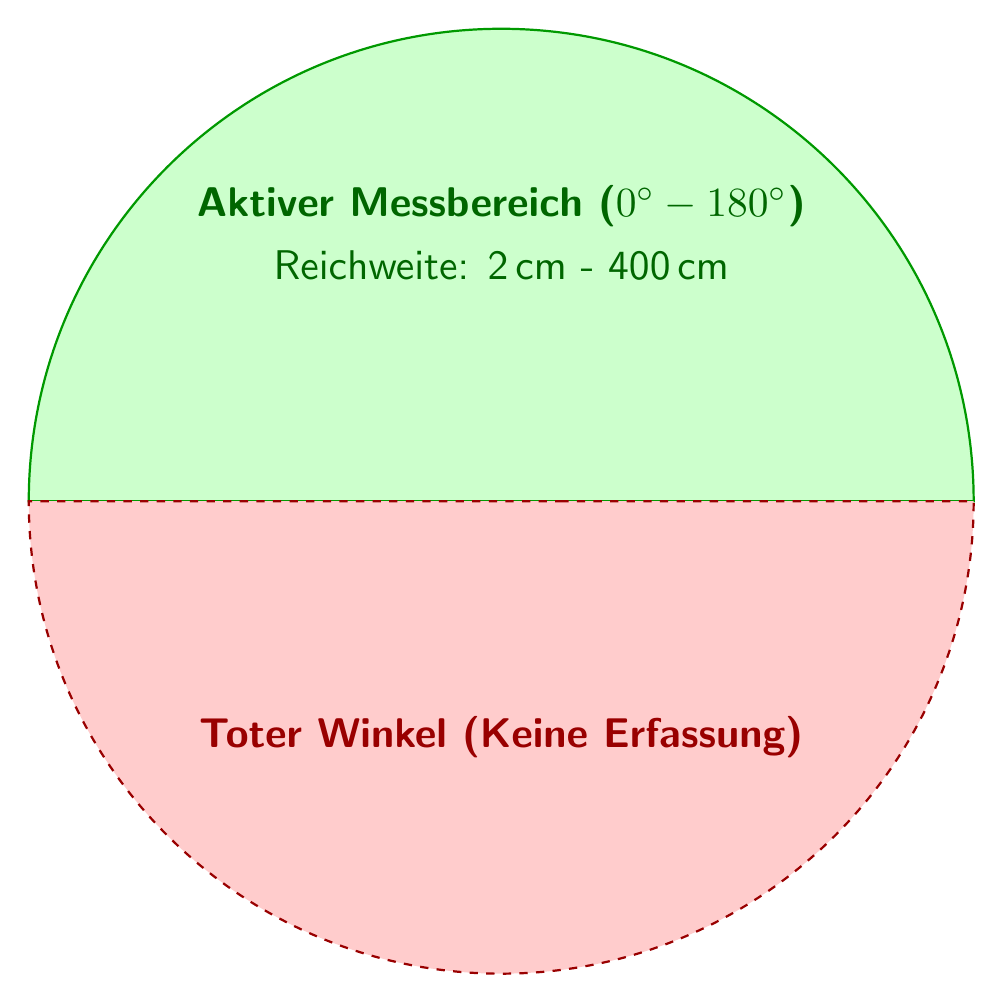
\begin{tikzpicture}[font=\sffamily, scale=1.5, transform shape]
	% Sensor in der Mitte
	\filldraw[fill=gray!50, draw=black, thick] (-0.5,-0.5) rectangle (0.5,0.5);
	\node at (0,0) {\textbf{Radar}};
	
	% Aktiver Bereich (oben)
	\filldraw[fill=green!20, draw=green!60!black, thick] (0.5,0) -- (4,0) arc (0:180:4) -- (-0.5,0) -- cycle;
	\node[text=green!40!black] at (0, 2.5) {\textbf{Aktiver Messbereich ($0^\circ - 180^\circ$)}};
	\node[text=green!40!black] at (0, 2) {Reichweite: 2\,cm - 400\,cm};
	
	% Toter Winkel (unten)
	\filldraw[fill=red!20, draw=red!60!black, thick, dashed] (0.5,0) -- (4,0) arc (360:180:4) -- (-0.5,0) -- cycle;
	\node[text=red!60!black] at (0, -2) {\textbf{Toter Winkel (Keine Erfassung)}};
\end{tikzpicture}
	\caption{Reichweite}
\end{figure}
In der oberen linken Ecke der Benutzeroberfläche befindet sich die Statusanzeige. Sie zeigt den aktuellen Systemstatus (\textit{,,SYSTEM OK''}), den exakten aktuellen Scan-Winkel in Grad sowie die berechnete Distanz zum nächsten Objekt in Zentimetern an. Das System erkennt Objekte zuverlässig in einer Distanz von ca. $2\,cm$ bis $40\,cm$. Über die $40\,cm$ hinaus werden Objekte auch noch erkannt, jedoch werden sie nichtmehr in der Benutzeroberfläche dargestellt, da die genaue Winkelpositionierung bei größerer Entfernung nicht mehr gegeben ist. 
